\documentclass[nooutcomes]{ximera}

\input{../preamble}
\author{Bobby Ramsey}
\license{Creative Commons Attribution-ShareAlike 4.0 International License}
\acknowledgement{}

\title{Applications of Systems}

 % for drawing cube in Optimization problem
\usetikzlibrary{quotes,arrows.meta}
\tikzset{
  annotated cuboid/.pic={
    \tikzset{%
      every edge quotes/.append style={midway, auto},
      /cuboid/.cd,
      #1
    }
    \draw [every edge/.append style={pic actions, densely dashed, opacity=.5}, pic actions]
    (0,0,0) coordinate (o) -- ++(-\cubescale*\cubex,0,0) coordinate (a) -- ++(0,-\cubescale*\cubey,0) coordinate (b) edge coordinate [pos=1] (g) ++(0,0,-\cubescale*\cubez)  -- ++(\cubescale*\cubex,0,0) coordinate (c) -- cycle
    (o) -- ++(0,0,-\cubescale*\cubez) coordinate (d) -- ++(0,-\cubescale*\cubey,0) coordinate (e) edge (g) -- (c) -- cycle
    (o) -- (a) -- ++(0,0,-\cubescale*\cubez) coordinate (f) edge (g) -- (d) -- cycle;
    \path [every edge/.append style={pic actions, |-|}]
    (b) +(0,-5pt) coordinate (b1) edge ["x"'] (b1 -| c)
    (b) +(-5pt,0) coordinate (b2) edge ["y"] (b2 |- a)
    (c) +(3.5pt,-3.5pt) coordinate (c2) edge ["x"'] ([xshift=3.5pt,yshift=-3.5pt]e)
    ;
  },
  /cuboid/.search also={/tikz},
  /cuboid/.cd,
  width/.store in=\cubex,
  height/.store in=\cubey,
  depth/.store in=\cubez,
  units/.store in=\cubeunits,
  scale/.store in=\cubescale,
  width=10,
  height=10,
  depth=10,
  units=cm,
  scale=.1,
}

\begin{document}
\begin{abstract}
  
\end{abstract}
\maketitle

%\begin{motivatingQuestions}\begin{itemize}
%	\item 
%	\item 
%	\item 
%\end{itemize}\end{motivatingQuestions}

%\typeout{************************************************}
%\typeout{Introduction}
%\typeout{************************************************}
\section{Introduction}
	Suppose a rectangle has width $w$ and length $l$, with area $24$ and perimeter $20$. The area of the rectangle is $wl$ and the perimeter is given by $2w + 2l$, 
	giving the following system of equations
	$$	\begin{cases}
			wl &= 24\\
			2w + 2l &= 20.
		\end{cases}	$$
	Since the first equation here is not a linear equation, this is a nonlinear system of equations. If we want to find the dimensions of the corresponding rectangle, we must solve
	this system. Since calculations of areas and volumes are nonlinear in general, situations involving geometric shapes often result in nonlinear systems of equations. 
	 
	To solve this system, we will start by dividing both sides of the second equation by $2$, to obtain the following equivalent system. 
	$$	\begin{cases}
			wl &= 24\\
			w + l &= 10.
		\end{cases}	$$
	If this second equation is satisfied, that means $l = 10-w$, which can be substituted into the top equation to eliminate the variable $l$.
	\begin{align*}
		wl &= 24\\
		w(10-w) &= 24\\
		10w- w^2 &= 24\\
		w^2 - 10w + 24 &=0\\
		(w-6)(w-4) &= 0.
	\end{align*}	
	The $w-6$ factor gives a solution of $w=6$, and the $w-4$ factor gives a solution of $w=4$.		
	
	Looking back at $l = 10-w$ we see that if $w=6$, then $l=10-6 = 4$ and if $w=4$ then $l = 10-4 = 6$.
	
	There are two possible rectangles: One with width $6$ and length $4$, and the other with width $4$ and length $6$.
		
%%\typeout{************************************************}
%%\typeout{Applications of Systems}
%%\typeout{************************************************}
\section{Applications of Systems}

	\begin{exercise}
		A rectangle is drawn in the first quadrant with one side along the $x$-axis, one side along the $y$-axis, the lower left corner at the origin, and upper right corner on the 
		graph of the equation $y=8-2x$. Denote this \emph{upper right} vertex as $(x,y)$. Find the coordinates of the point $(x,y)$ 
		if the area of the rectangle is $\frac{15}{2}$.
		\begin{image}
			\begin{tikzpicture}
				\begin{axis}[
					xmin=-0.5, xmax=4.5, ymin=-0.5,ymax=10.5,    
					axis lines =middle, 
					every axis y label/.style={at=(current axis.above origin),anchor=south},
					every axis x label/.style={at=(current axis.right of origin),anchor=west},
					xtick={0,...,4}, ytick={0,2,...,10},
					grid=major, %width=4in, height=3in,
					grid style={dashed, gray!40} 					
					]
					\addplot[color=penColor, very thick, smooth, domain=-0.5:4.25]{8-2*x} node[pos=0.25, color=penColor2, above right]{\Large{$y=8-2x$}};										\draw[fill=penColor3!10!white](axis cs:0,0) rectangle (axis cs:2, 4);					
					\addplot+[soliddot, color=penColor3] coordinates {(2,4)}  node [above right] {$(x,y)$};
				\end{axis}
			\end{tikzpicture}
		\end{image}

		\begin{explanation}
			Since $(x,y)$ are the coordinates of the upper right vertex, this tells us that $x$ and $y$ are both positive.
			It also tells us that the distance from the $x$-axis is $y$, and the distance from the $y$-axis is $x$.
			In other words, the height of the rectangle is just $y$, and the width of the rectangle is $x$. In terms of $x$ and $y$,
			the area is given by $xy$, giving us one equation $xy = \frac{15}{2}$. 
			
			Since the upper right corner $(x,y)$ is on the graph of the line, we also know that $y=8-2x$. This leaves us with the following system:
			This gives a system of nonlinear equations
			$$	\begin{cases}
				xy &= \frac{15}{2}\\
				y &= 8-2x.
			\end{cases}	$$	
			
			This bottom equation is already solved for $y$, so the easiest way to eliminate a variable would be to substitute it into the $y$ in the top equation.
			\begin{align*}
				xy &= \frac{15}{2}\\
				x(8-2x) &= \frac{15}{2}\\
				8x - 2x^2 &= \frac{15}{2}\\
				2x^2 - 8x &= - \frac{15}{2}\\
				x^2 - 4x &= - \frac{15}{4}.
			\end{align*}
			We'll solve this equation by completing the square.
			\begin{align*}
				x^2 - 4x &= - \frac{15}{4}\\
				x^2 - 4x + 4&= - \frac{15}{4} + 4\\
				x^2 - 4x + 4&= \frac{1}{4}\\
				(x-2)^2 &= \frac{1}{4}\\
				x-2 &= \pm \sqrt{\frac{1}{4}}\\
				x-2 &= \pm \frac{1}{2}\\
				x &= 2 \pm \frac{1}{2}\\
				x &= \frac{3}{2}, \frac{5}{2}\\
			\end{align*}	
			
			If $x=\frac{3}{2}$ then $y=8-2\left(\frac{3}{2}\right) = 5$, and if $x=\frac{5}{2}$ then $y=8-2\left(\frac{5}{2}\right) = 3$.
			
			There are two possibilities. One has coordinates $\left( \frac{3}{2}, 5 \right)$ and the other has coordinates $\left( \frac{5}{2}, 3 \right)$.
		\end{explanation}
	\end{exercise}


	\begin{exercise}
		A right triangle has hypotenuse of length $13 m$ and area $30 m^2$. Find the lengths of the two legs of the triangle.
		\begin{image}[2in]
			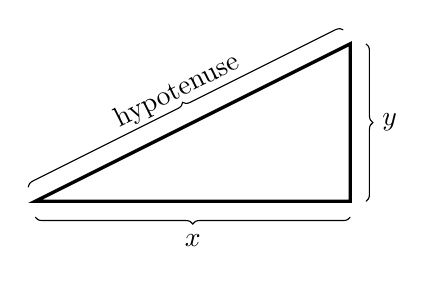
\begin{tikzpicture}
				\coordinate (C) at (0,2);
				\coordinate (D) at (4,2);
				\coordinate (E) at (4,4);
				\tkzMarkRightAngle(C,D,E)
				\draw[decoration={brace,mirror,raise=.2cm},decorate,thin] (0,2)--(4,2);
				\draw[decoration={brace,mirror,raise=.2cm},decorate,thin] (4,2)--(4,4);
				\draw[decoration={brace,raise=.2cm},decorate,thin] (0,2)--(4,4);
				\draw[very thick] (D)--(E)--(C)--cycle;
				\node at (2,2-.5) {$x$};
				\node at (4+.5,3) {$y$};
				\node[rotate=26.5] at (2-.2,3+.4) {hypotenuse};
			  \end{tikzpicture}
		\end{image}
		\begin{explanation}
			
			Since this is a right triangle, the Pythagorean Theorem tells us that $x^2 + y^2 = 13^2 = 169$.
			The area of a triangle is given by $\frac{1}{2}\times \text{base} \times \text{height}$ which means
			$\frac{1}{2}xy = 30$, or equivalently $xy = 60$.

			This gives a system of nonlinear equations
			$$	\begin{cases}
				x^2+y^2 &= 169\\
				xy &= 60.
			\end{cases}	$$
			
			A direct way to solve this system of equations would be to solve the bottom equation for $y$, giving $y = \frac{60}{x}$, and substitute this into the top equation
			eliminating the $y$ variable. After simplification that will yield a degree $4$ polynomial equation to solve for $x$. Instead of following that method, we will make 
			use of a different algebraic trick.
			
			We know that there is a difference between $x^2 + y^2$ and $(x+y)^2$. If we multiply out $(x+y)^2$ we get $x^2 + 2xy + y^2$. That means if we add $2xy$
			to $x^2 + y^2$, it becomes $(x+y)^2$. In order to do that, we need to know the value of $2xy$ to add to the other side of our top equation,
			Notice that the bottom equation of our system $xy=60$ means that $2xy = 2(60)=120$. If the bottom equation is satisfied, the top equation can be
			rewritten as:
			\begin{align*}
				x^2 + y^2 &= 169\\
				x^2 + y^2 + 2xy &= 169 + 2xy\\
				x^2 + 2xy + y^2 &= 169 + 120\\				
				\left( x + y \right)^2 &= 289.
			\end{align*}
			Since neither $x$ nor $y$ can be negative, $x+y = \sqrt{289} = 17$.
			Our system of equations is equivalent to:
			$$	\begin{cases}
				x + y &= 17\\
				xy &= 60.
			\end{cases}	$$
			
			Now that we've been able to simplify the first equation, we will proceed with substitution as mentioned above. If $y =\frac{60}{x}$ is satisfied, then the top
			equation gives:
			\begin{align*}
				x + y &= 17\\
				x + \frac{60}{x} &= 17\\
				x\left( x + \frac{60}{x}\right) &= x(17)\\
				x^2 + 60 &= 17x\\
				x^2 - 17x + 60 &= 0\\
				(x-12)(x-5) &= 0.
			\end{align*}				
			The $x-12$ factor yields a solution of $x=12$, and the $x-5$ factor gives a solution of $x=5$. Using $y=\frac{60}{x}$ we find that if
			$x=12$ then $y = \frac{60}{12}=5$, and if $x=5$ then $y=\frac{60}{5} = 12$.
			
			The two legs of the triangle have lengths $5 m$ and $12 m$.
					
		\end{explanation}
	\end{exercise}

	\begin{exercise}
		Suppose we have a box with square base, as illustrated below, constructed to have volume $8 cm^3$ and surface area $24 cm^2$. 
		Call the side-lengths of the base as $x$, and the height of the box as $y$.
		\begin{image}
			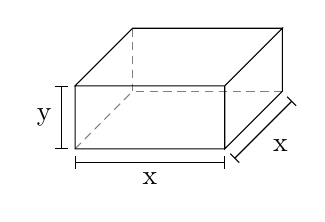
\begin{tikzpicture}
				\pic {annotated cuboid={width=95, height=40, depth=95, scale=.02, units=cm}};
			\end{tikzpicture}
		\end{image}
		Find the dimensions of the box.
		
		\begin{explanation}	
			We know that the volume of the box is given by $x^2y$ ($\text{length} \times \text{width} \times \text{height}$), giving the nonlinear equation
			 $x^2y = 8$. The surface of the box consists of six rectangles. The top and bottom each have area $x^2$, and the four sides each have 
			 area $xy$. The full surface area of the box is given by $2x^2 + 4xy$.
			This setup gives us a system of two nonlinear equations with two unknowns:
			$$	\begin{cases}
					x^2 y &= 8\\
					2x^2 + 4xy &= 24.
				\end{cases}	$$
			If we want to find the dimensions of the box, we will have to solve this system of equations.
			
			As you have seen in the previous section, solving systems of nonlinear equations involves finding a way to eliminate one of the variables through 
			performing operations on the two equations and/or substutition. In the case of these equations, notice that the variable $y$ only occurs in a single
			term in each equation. In the top equation there is an $x^2 y$ term, while in the bottom equation there is an $xy$ term. These are not 
			``like terms'', so we will need to deal with that. Let us begin by multiplying both sides of the second equation by $x$. This gives the system
			$$	\begin{cases}
					x^2 y &= 8\\
					2x^3 + 4x^2y &= 24x.
				\end{cases}	$$
			Since no solution has $x$-coordinate equal to $0$, this system is equivalent to the original one. This modification has given that the $y$ variable 
			appears in like terms in boh equations. Substituting $x^2y = 8$ into the new bottom equation gives:
			\begin{align*}
				2x^3 + 4x^2 y &= 24x\\
				2x^3 + 4\left(x^2 y\right) &= 24x\\
				2x^3 + 4\left(8\right) &= 24x\\
				2x^3 + 32 &= 24x\\
				2x^3 - 24x + 32 &= 0\\
				x^3 - 12x + 16 &= 0.
			\end{align*}
			That is, if the $x^2y=8$ equation is satisfied, then the bottom equation of the system is equivalent to $x^3-12x+16=0$. This is a polynomial 
			equation in the single variable, $x$.
			
			Notice that $2^3-12(2)+16 = 8 -24+16 = 0$. That means $x=2$ is a solution to this cubic equation, and that $x-2$ is a factor of the 
			polynomial $x^3-12x+16$. By long-division we can find that $x^3-12x+16 = (x-2)(x^2+2x-8)$. Since $x^2+2x-8 = (x+4)(x-2)$ we see
			that $x^3-12x+16 = (x-2)^2(x+4)$. The zeroes of this polymial are $x=2$ and $x=-4$. Since $x$ represents a length of the side of the box, 
			the $x=-4$ solution is extraneous and should be dropped.
			
			The only solution to the system has $x=2$. Looking back at the first equation of the system:
			\begin{align*}
				x^2 y &= 8\\
				(2)^2y &= 8\\
				4y &=8\\
				y &= 2.
			\end{align*}
			The solution is for $(x,y) = (2,2)$. Since the question asks us to find the dimensions of the box, we say that the box is 
			$2 cm \times 2 cm \times 2 cm$. That is, it's a cube with side length $2 cm$.
	
		\end{explanation}
	\end{exercise}	


	


\end{document}
